%%%%%%%%%%%%%%%%%%%%%%%%%%%%%%%%%%%%%%%%%
% Beamer Presentation
% LaTeX Template
% Version 1.0 (10/11/12)
%
% This template has been downloaded from:
% http://www.LaTeXTemplates.com
%
% License:
% CC BY-NC-SA 3.0 (http://creativecommons.org/licenses/by-nc-sa/3.0/)
%
%%%%%%%%%%%%%%%%%%%%%%%%%%%%%%%%%%%%%%%%%

%----------------------------------------------------------------------------------------
%	PACKAGES AND THEMES
%----------------------------------------------------------------------------------------

\documentclass{beamer}

\definecolor{sblue}  {RGB}{20,90,170}
\definecolor{lgreen} {RGB}{10,220,50}
\definecolor{lred}   {RGB}{220,0,0}

\newcommand{\E}{\mathbb{E}}
\newcommand{\R}{\mathbb{R}}
\newcommand{\N}{\mathbb{N}}
\newcommand{\I}{\mathbb{I}}
\newcommand{\tpsi}{\tilde{\psi}}
\newcommand{\hpsi}{\hat{\psi}}
\newcommand{\tPsi}{\tilde{\Psi}}
\newcommand\given[1][]{\:#1\vert\:}
\newcommand{\var}{\mathrm{\mathbb{V}ar}}
\newcommand{\cov}{\mathrm{\mathbb{C}ov}}
\newcommand{\corr}{\mathrm{corr}}
\newcommand{\vect}[1]{\boldsymbol{#1}}
\newcommand{\vectg}[1]{\boldsymbol{#1}}
\newcommand{\bd}[1]{\boldsymbol{#1}}
\newcommand{\idx}[3][]{{#2}^{(#3)}_{#1}}
\newcommand{\bidx}[3][]{\bd{#2}^{(#3)}_{#1}}
\newcommand{\aidx}[3][]{#2^{\langle#3\rangle}_{#1}}
\newcommand{\col}[1]{\textcolor{lred}{#1}}

\usepackage{tikz}
\usepackage{graphicx}
\graphicspath{{./img/}}


\mode<presentation> {

% The Beamer class comes with a number of default slide themes
% which change the colors and layouts of slides. Below this is a list
% of all the themes, uncomment each in turn to see what they look like.

%\usetheme{default}
%\usetheme{AnnArbor}
%\usetheme{Antibes}
%\usetheme{Bergen}
%\usetheme{Berkeley}
%\usetheme{Berlin}
%\usetheme{Boadilla}
%\usetheme{CambridgeUS}
%\usetheme{Copenhagen}
%\usetheme{Darmstadt}
%\usetheme{Dresden}
%\usetheme{Frankfurt}
%\usetheme{Goettingen}
%\usetheme{Hannover}
%\usetheme{Ilmenau}
%\usetheme{JuanLesPins}
%\usetheme{Luebeck}
\usetheme{Madrid}
%\usetheme{Malmoe}
%\usetheme{Marburg}
%\usetheme{Montpellier}
%\usetheme{PaloAlto}
%\usetheme{Pittsburgh}
%\usetheme{Rochester}
%\usetheme{Singapore}
%\usetheme{Szeged}
%\usetheme{Warsaw}

% As well as themes, the Beamer class has a number of color themes
% for any slide theme. Uncomment each of these in turn to see how it
% changes the colors of your current slide theme.

%\usecolortheme{albatross}
%\usecolortheme{beaver}
%\usecolortheme{beetle}
%\usecolortheme{crane}
%\usecolortheme{dolphin}
%\usecolortheme{dove}
%\usecolortheme{fly}
%\usecolortheme{lily}
%\usecolortheme{orchid}
%\usecolortheme{rose}
%\usecolortheme{seagull}
%\usecolortheme{seahorse}
%\usecolortheme{whale}
%\usecolortheme{wolverine}

%\setbeamertemplate{footline} % To remove the footer line in all slides uncomment this line
 %\setbeamertemplate{footline}[page number] % To replace the footer line in all slides with a simple slide count uncomment this line

\setbeamertemplate{navigation symbols}{} % To remove the navigation symbols from the bottom of all slides uncomment this line
}

\usepackage{graphicx} % Allows including images
\usepackage{booktabs} % Allows the use of \toprule, \midrule and \bottomrule in tables

%----------------------------------------------------------------------------------------
%	TITLE PAGE
%----------------------------------------------------------------------------------------

\title[AAEs \& WAEs]{Adversarial Auto-Encoders (AAEs) and \\ Wasserstein Auto-Encoders (WAEs)}

\author[A. Lin \and M. Yu]{Alex Lin \and Melissa Yu} 
\institute[Harvard University]{Harvard University}
\date{\today}

\begin{document}

\begin{frame}
\titlepage 
\end{frame}

\section{Introduction} 

\begin{frame}{Jensen-Shannon divergence}
	Minimize Jensen-Shannon divergence between true data distribution $p_d$ and generative model $p_g$:
	\[
	\min_G \mathcal{D}_{JS}(p_d(x) \vert\vert p_g(x))
	\]
	
	where
	\[
	\mathcal{D}_{JS}(p_d(x) \vert\vert p_g(x)) = 
	\frac{1}{2} \mathcal{D}_{KL}(p_d \vert\vert \frac{p_d + p_g}{2}) +
	\frac{1}{2} \mathcal{D}_{KL}(p_g \vert\vert \frac{p_d + p_g}{2})
	\]
\end{frame}

\begin{frame}{Generative Adversarial Networks (GANs)}
	Minimizing JSD corresponds to finding best $G$ when $D$ is optimal
	\[
	\min_G \max_D V(D, G) = \E_{p_d(x)} [\log D(x)] + \E_{p_z(z)} [\log (1 - D(G(z)))]
	\]
	
	Min-max game between 2 neural networks
	\begin{itemize}
		\item generator $G(z)$: prior $p_z(z)$ and likelihood $p(x\given z)$
		\item discriminator $D(x)$: predicts probability $x$ comes from $p_d$, not $p_g$
	\end{itemize}
\end{frame}

\begin{frame}{VAEs}
	Encoder $q(z\given x)$, decoder $p(x\given z)$. Prior on latent codes $p(z)$.
	
	\begin{align*}
	\min_q \ & \E_{q(z\given x)} [-\log p(x\given z)] + \mathcal{D}_{KL}(q(z\given x) \ \vert\vert \ p(z)) \\
	&= \text{Reconstruction} + \text{Regularization}
	\end{align*}
\end{frame}

\begin{frame}{Adversarial Auto-encoders (AAEs)}
	\begin{itemize}
	\item Aggregated posterior
\begin{equation*}
q(z) = \int_{x} q(z\given x) p_d(x) dx
\end{equation*}

	\item Replaces VAE's $\mathcal{D}_{KL}(q(z\given x) \ \vert\vert \ p(z))$ regularizer with $\mathcal{D}_{JS}(q(z) \ \vert\vert \ p(z))$
	\end{itemize}
\end{frame}

\begin{frame}{AAE: Adversarial Networks}
	\begin{itemize}
		\item Directly minimizing $\mathcal{D}_{JS}(p(z) \ \vert\vert \ q(z))$ is intractable
		
		\item $\Rightarrow$ Attach adversarial network on top of $z$
		\begin{itemize}
			\item Encoder of autoencoder is also generator of adversarial network 
			\[G(z) = q(z\given x)\]
			
			\item Discriminator $D$ distinguishes $p(z)$ (positive samples) from $q(z)$ (negative samples)
		\end{itemize}
	\end{itemize}
\end{frame}

\begin{frame}{AAE}
	\begin{center}
		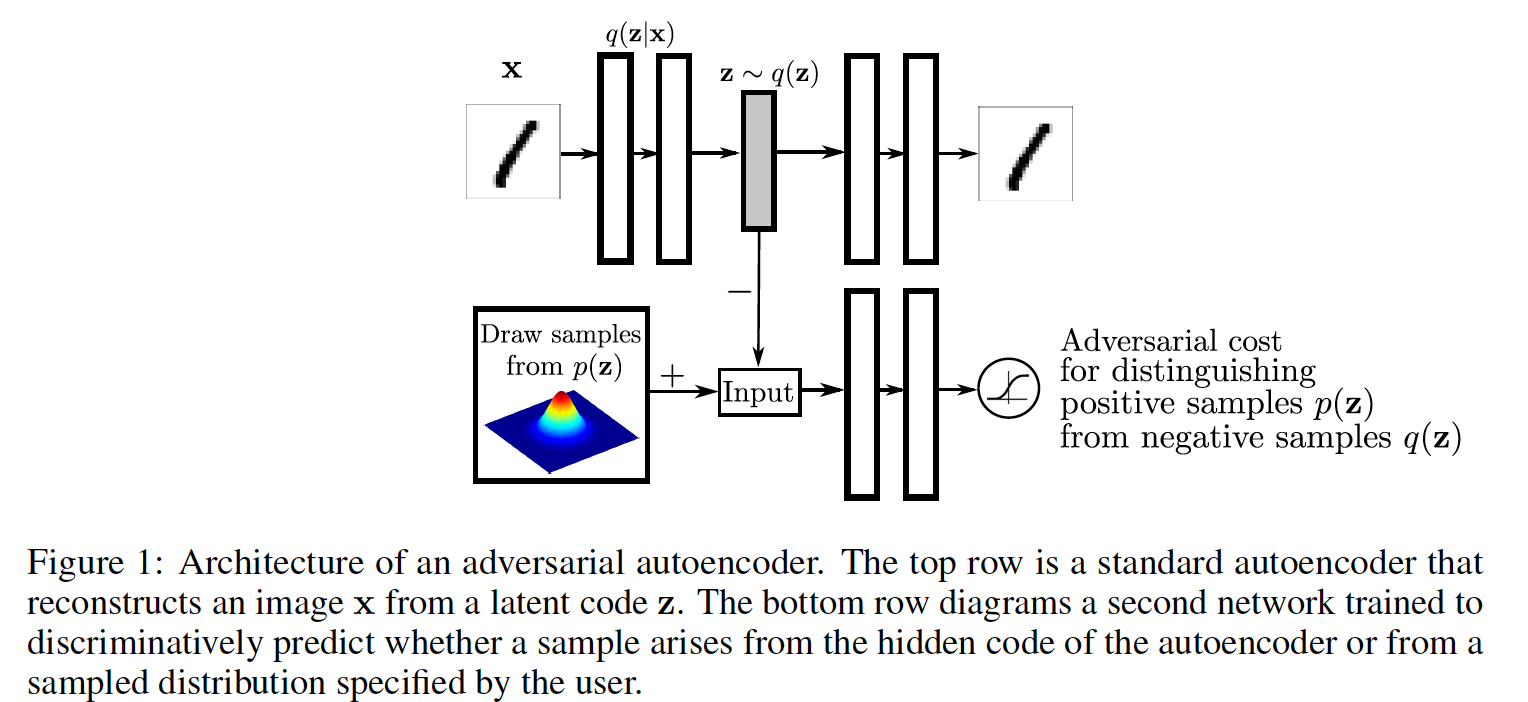
\includegraphics[width=0.9\linewidth]{AAE}
	\end{center}
\end{frame}

\begin{frame}{AAE}
	Trained by alternately minimizing reconstruction error and training adversarial network
	\begin{enumerate}
		\item \textit{Reconstruction phase.} 
		Encoder $q$ and decoder $p$ are trained to minimize reconstruction error:
		\begin{equation}
		\min_{q, p} \ \E_{q(z\given x)} [-\log p(x\given z)]
		\end{equation}
		
		\item \textit{Regularization phase.} 
		Adversarial network is trained on GAN objective:
		\begin{equation*}
		\min_q \max_{D} \ \E_{p(z)} [\log D(z)] + \E_{q(z\given x)} [\log (1 - D(z))] 
		\end{equation*}
		
	\end{enumerate}
\end{frame}

\begin{frame}{Choice of Encoder $q$}
	\begin{itemize}
		\item Deterministic: $q$ is deterministic function of $x$
		\begin{itemize}
			\item may not produce smooth mapping; empirical distribution of data is fixed by training set
		\end{itemize}
	
		\item Gaussian posterior: $q$ is Gaussian distribution whose parameters are predicted by encoder network
		\[
		z \sim \mathcal{N}(\mu(x), \sigma(x))
		\]
		\item Universal approximator posterior
	\end{itemize}
\end{frame}

\begin{frame}{Encoder (cont.)}
	\begin{itemize}
		\item Gaussian posterior + universal approximator posterior give network additional sources of stochasticity that could help it in the adversarial regularization stage by smoothing out $q(z)$.
		
		\item In practice, authors obtain similar test likelihoods for all 3 choices.
	\end{itemize}
\end{frame}

\begin{frame}
\frametitle{WAE Paper}
\begin{center}
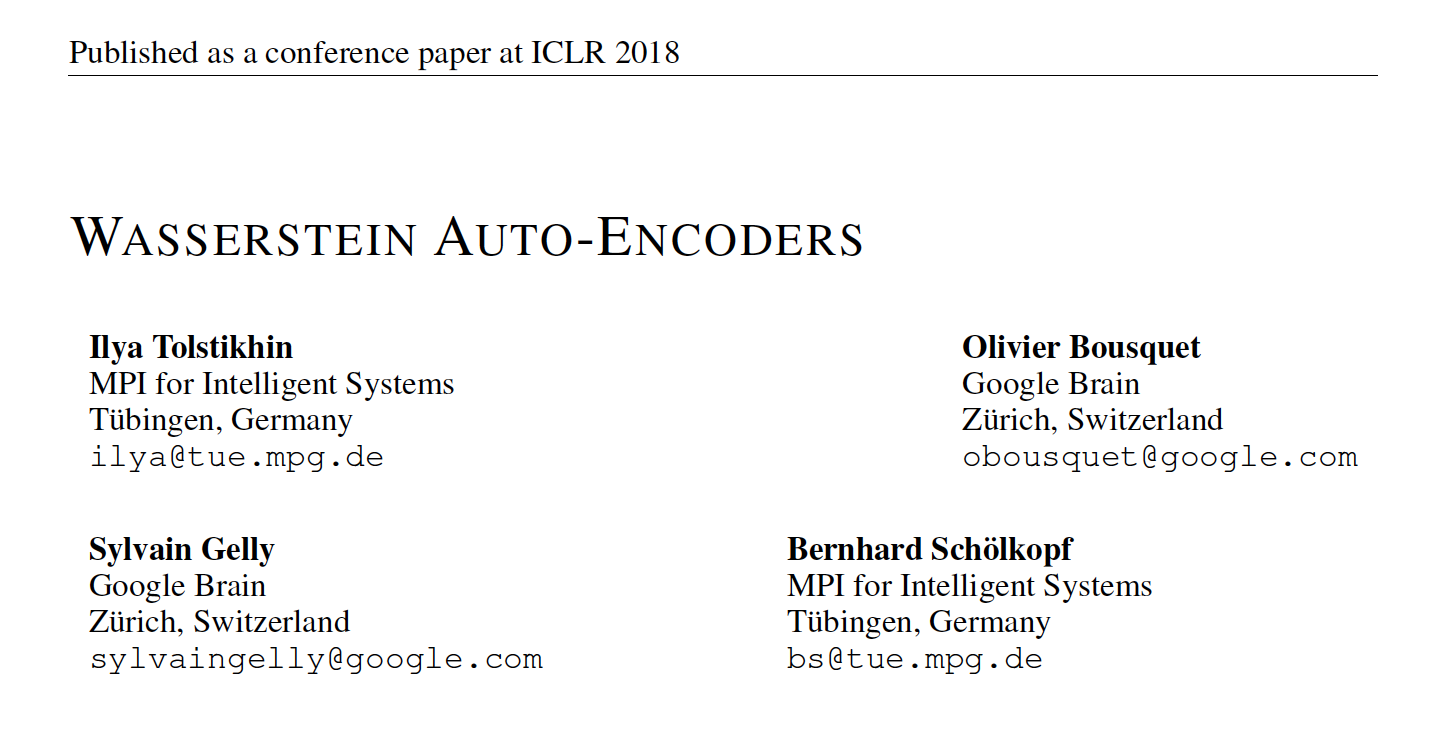
\includegraphics[scale=0.5]{wae-paper}
\end{center}
\end{frame}

\begin{frame}
\frametitle{A Quick Review of VAEs}
\begin{itemize}
\item Let our data $x_1, \ldots, x_n \in \mathcal{X}$ be distributed according to $P_X$.
\pause 

\item Goal of generative modeling is to find a model $G$ with $P_G : \mathcal{X} \to [0, 1]$ that minimizes a specified distance $D(P_X, P_G)$.  
\pause

\item \col{Variational Auto-Encoders} (VAEs) seek to minimize 
\begin{align*}
D_{KL}(P_X, P_G) = \underbrace{-\E_{P_X}[\log P_G(X)]}_{\text{\col{negative log-likelihood}}} + \underbrace{\E_{P_X}[\log P_X(X)]}_{\text{entropy of data}}
\end{align*} 
\pause

\item The NLL cannot be optimized directly, so VAEs use an \col{upper bound}.
\begin{align*}
 & NLL \leq \inf_{\underbrace{Q(Z \vert X) \in \mathcal{Q}}_{\text{min over all encoders}}} -\E_{P_X}[\underbrace{\E_{Q(Z \vert X)}[\log P_G(X \vert Z)]}_{\text{reconstruction loss}} - \underbrace{D_{KL}(Q(Z \vert X), P_Z)}_{\text{regularization loss}}]
\end{align*}
\pause

\item Take-Away: VAEs \col{minimize an upper bound on KL divergence} between the data and the model.

\end{itemize}
\end{frame}

\begin{frame}
\frametitle{Using Wasserstein instead of KL}
\begin{itemize}
\setlength\itemsep{1em}
\item Alternative way to measure distance between probability distributions
\pause

\item Aka Earth Mover's Distance, Kantorovich-Rubinstein Metric, Optimal Transfer Plan
\pause

\item Defined with respect to a cost function $c : \mathcal{X} \times \mathcal{X} \to \R_{+}$ as 
\begin{align*}
W_c(P_X, P_Y) = \inf_{\Gamma \in \mathcal{P}(X \sim P_X, Y \sim P_Y)} \E_{(X, Y) \sim \Gamma} [c(X, Y)]
\end{align*}
where $\Gamma(x, y)$ is the "transport plan".

\begin{center}
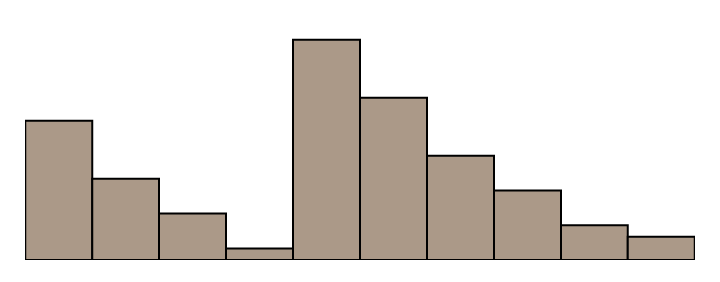
\includegraphics[scale=0.4]{discrete-em1}
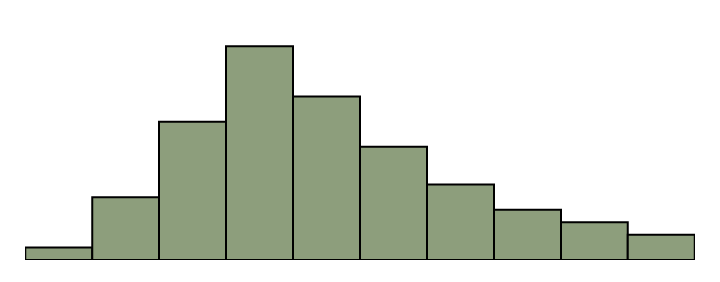
\includegraphics[scale=0.4]{discrete-em2}
\end{center}
\end{itemize}
\end{frame}

\begin{frame}
\frametitle{Using Wasserstein instead of KL}
\begin{itemize}
\setlength\itemsep{1em}

\item The objective is 

\begin{align*}
W_c(P_X, P_Y) = \inf_{\Gamma \in \mathcal{P}(X \sim P_X, Y \sim P_Y)} \E_{(X, Y) \sim \Gamma} [c(X, Y)]
\end{align*}

\pause

\begin{center}
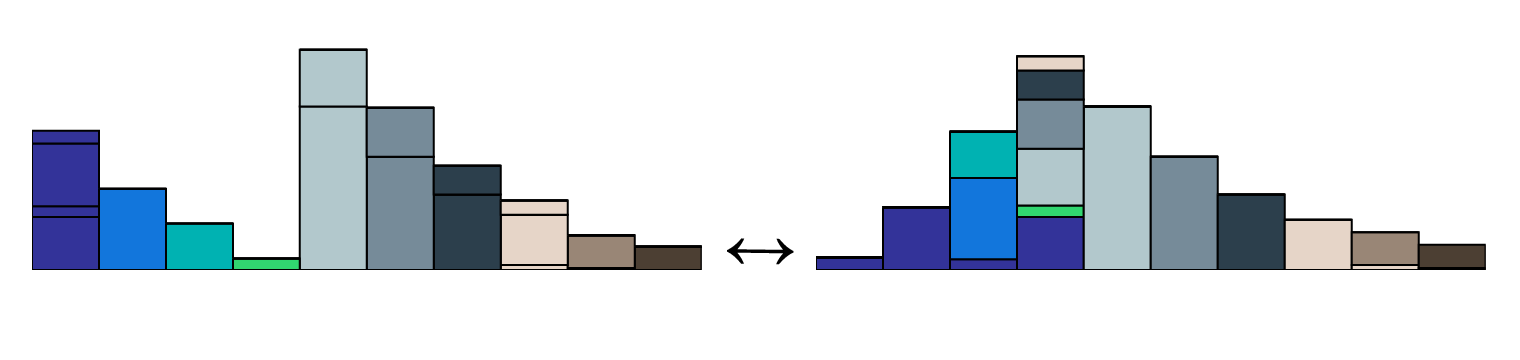
\includegraphics[scale=0.4]{discrete-em3}
\end{center}

\pause 

\item $\Gamma$ must be some joint distribution of $X, Y$ because 
\begin{itemize}
\item $\int_{x} \Gamma(x, y) dx = P_X(x) \Rightarrow $ Total earth leaving $x$ = total earth at $x$  
\item $\int_{y} \Gamma(x, y) dy = P_Y(y) \Rightarrow $ Total earth entering $y$ = total earth at $y$
\end{itemize}

\end{itemize}
\end{frame}

\begin{frame}
\frametitle{Wasserstein Auto-Encoder}
\begin{itemize}
\setlength\itemsep{1em}
\item Consider a latent space $\mathcal{Z}$ with prior $P_Z$.  We want to find a model (i.e. decoder) $G: \mathcal{Z} \to \mathcal{X}$ that minimizes the \col{Wasserstein distance}
\begin{align*}
W_c(P_X, P_G) = \inf_{\Gamma \in \mathcal{P}(X \sim P_X, Y \sim P_G)} \E_{(X, Y) \sim \Gamma} [c(X, Y)]
\end{align*}

\pause

\item \textbf{[Bousquet et al. (2017)]}  This is equivalent to minimizing 
\begin{align*}
W_c(P_X, P_G) = \inf_{\underbrace{Q: Q_Z = P_Z}_{\text{min over encoders with marginal $P_Z$}}} \E_{P_X} \underbrace{\E_{Q(Z \vert X)} [c(X, G(Z)]}_{\text{reconstruction cost}}
\end{align*}
where $Q_Z = \int Q(Z \vert X) P_X(X) dX$.  
\end{itemize}
\end{frame}

\begin{frame}
\frametitle{Wasserstein Auto-Encoder}
\begin{itemize}
\item The \col{WAE objective} relaxes the constraint $Q_Z = P_Z$ by adding a penalty.  It minimizes
\begin{align*}
D_{WAE}(P_X, P_G) =  \inf_{Q(Z \vert X) \in \mathcal{Q}} \E_{P_X} \E_{Q(Z \vert X)} [c(X, G(Z)]+ \lambda \cdot \mathcal{D}_Z(Q_Z, P_Z)
\end{align*}
where $\mathcal{D}$ is some divergence and $\lambda$ is some regularization parameter. 

\pause

\item Claims to fix \col{blurriness issue} of VAEs

\begin{center}
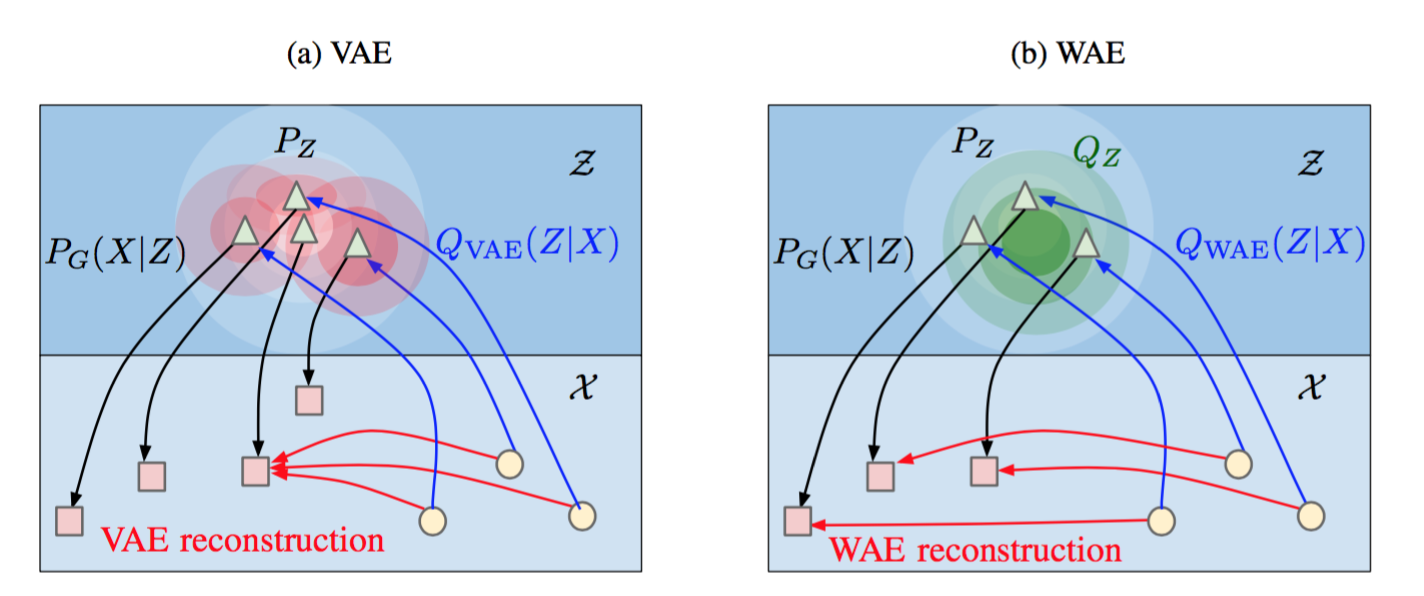
\includegraphics[scale=0.4]{wae-vae}
\end{center}

\end{itemize}
\end{frame}

\begin{frame}
\frametitle{Wasserstein Auto-Encoder}
\begin{itemize}
\item The \col{WAE objective} minimizes
\begin{align*}
D_{WAE}(P_X, P_G) =  \inf_{Q(Z \vert X) \in \mathcal{Q}} \E_{P_X} \E_{Q(Z \vert X)} [c(X, G(Z))]+ \lambda \cdot \mathcal{D}_Z(Q_Z, P_Z)
\end{align*}
\pause

\item There are two sources of customization.  
\pause
\begin{enumerate}
\item Choose \col{divergence} between $Q_Z$ and $P_Z$.

\pause
\begin{center}
\begin{tabular}{  c || c  }
 \hline \hline 
 WAE-GAN & WAE-MMD \\ 
 \hline 
 $\mathcal{D}_Z = D_{JS}$ & $\mathcal{D}_Z = MMD_k$ \\  
 Introduce adversarial & Use unbiased \\
 discriminator in $\mathcal{Z}$ & U-statistic estimator \\ 
 \hline \hline   
\end{tabular}
\end{center}

\pause
\item Choose \col{reconstruction cost} function $c$.  
\begin{itemize}
\pause
\item If $c(x, x') = \| x - x' \|_2^2$, then WAE-GAN is equivalent to AAE

\pause
\item Theoretical justification of AAE as minimizing 2-Wasserstein distance
\end{itemize}

\end{enumerate}
\end{itemize}
\end{frame}

\begin{frame}
\frametitle{Experiments}
\begin{itemize}
\setlength\itemsep{1em}
\item Test VAE, WAE-GAN, WAE-MMD on MNIST and CelebA

\item Record Frechet Inception Distance (FID) to assess quality of images

\begin{center}
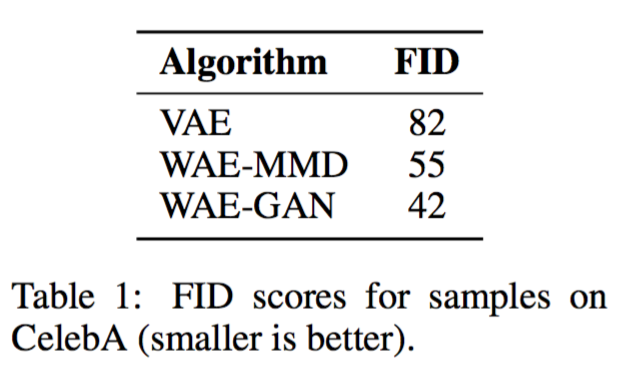
\includegraphics[scale=0.5]{experiments}
\end{center}

\end{itemize}
\end{frame}

\begin{frame}
\frametitle{Extensions}
\begin{center}
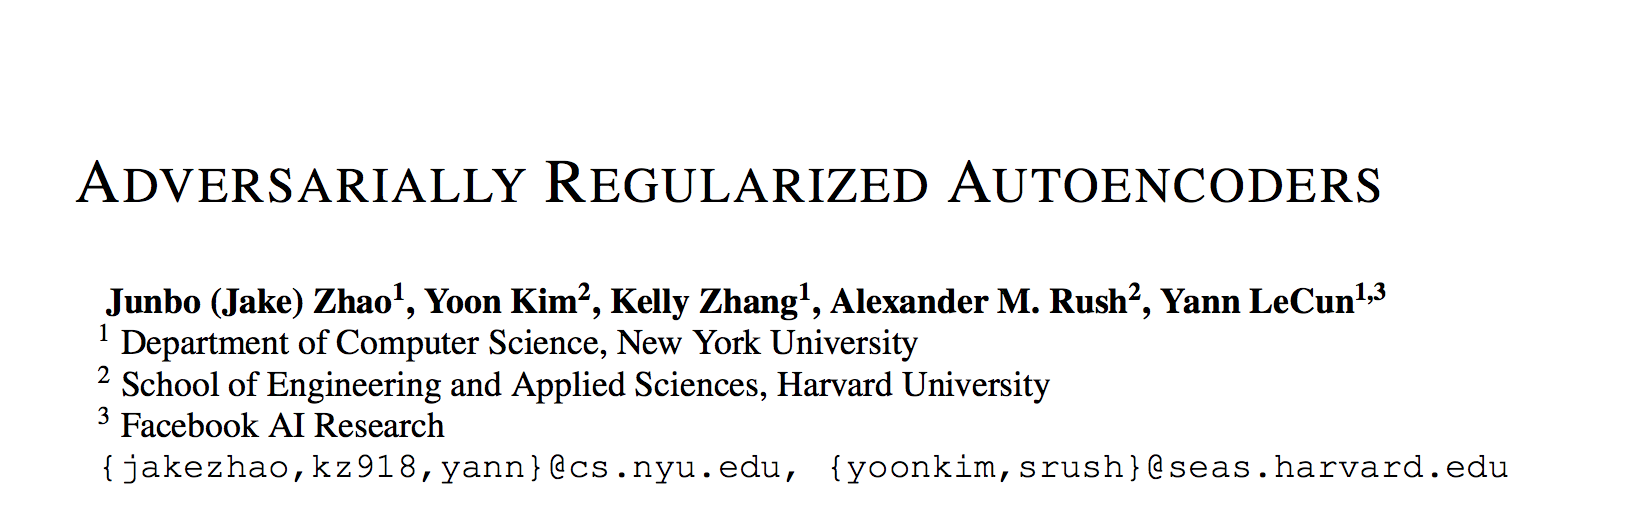
\includegraphics[scale=0.3]{paper1} \\ 
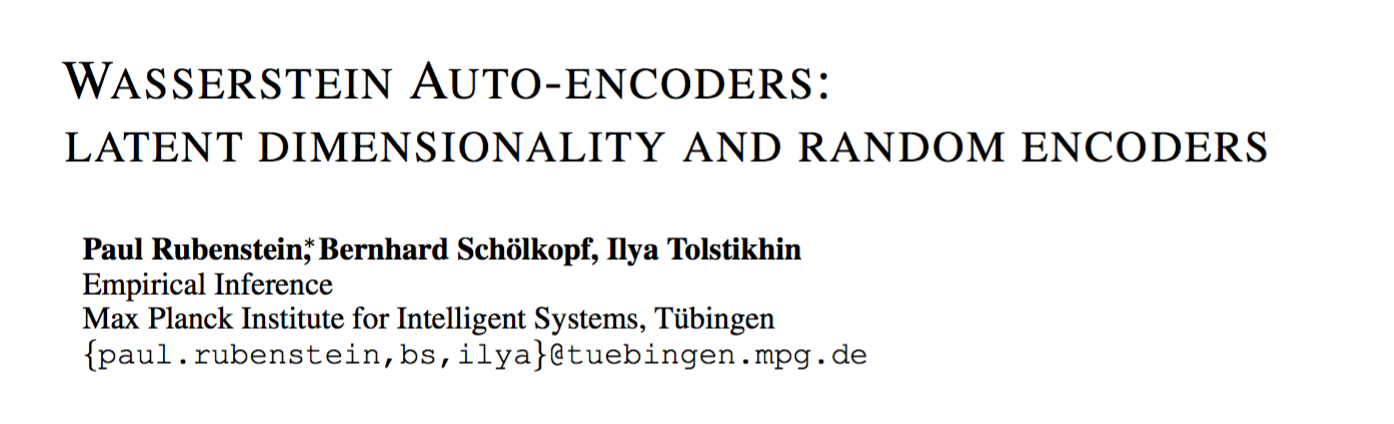
\includegraphics[scale=0.3]{paper2} \\
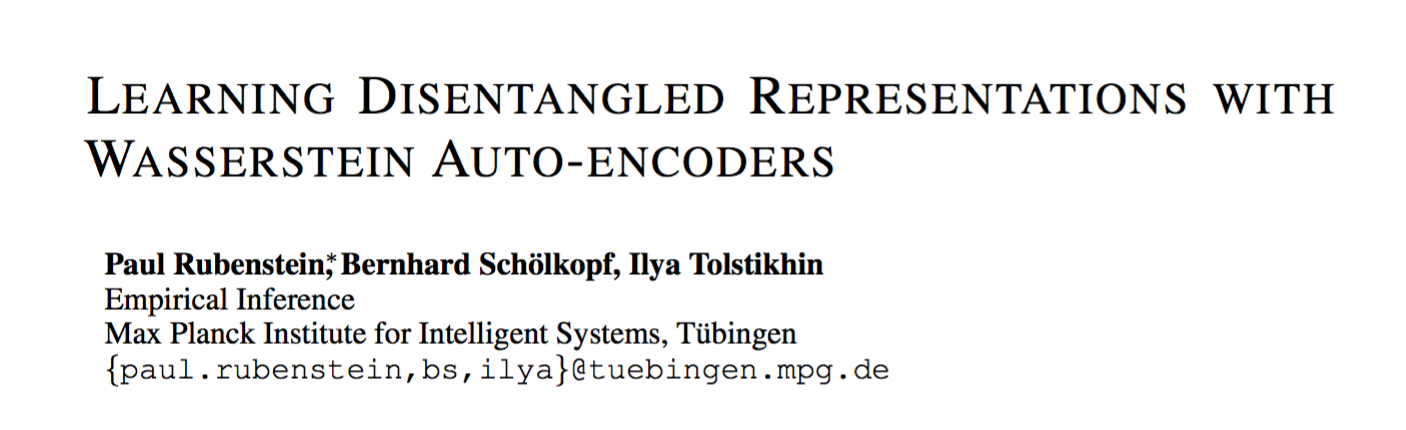
\includegraphics[scale=0.3]{paper3}
\end{center}
\end{frame}

\begin{frame}
\frametitle{Our Project}
\begin{itemize}
\setlength\itemsep{1em}
\item Build on work of Zhao et. al (2018) in applying WAEs to text

\pause 
\item Semi-Supervised Learning for transfering between different styles of English

\begin{itemize}
\pause
\item Shakespearean English vs. Modern English
\begin{center}

\includegraphics[scale=0.4]{shakespeare}
\end{center}

\pause
\item Formal English vs. Informal English
\begin{center}
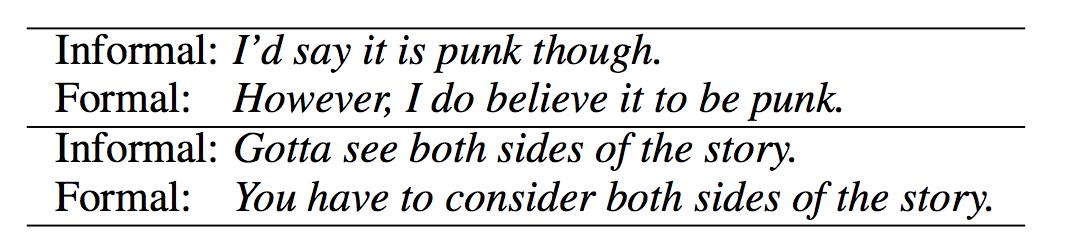
\includegraphics[scale=0.4]{informal}
\end{center}
\end{itemize}
\end{itemize}
\end{frame}

\end{document} 